\section{Kooperations-Situation mit anderen Hochschulen (ME)}
\label{section_kooperations_situation}

Das Kooperationsverhältnis mit anderen Hochschulen, Verbänden und Unternehmen spielt auch an der Hochschule Emden/Leer eine sehr entscheidende Rolle, da durch die Kooperation verschiedene Services zur Verfügung gestellt werden.

\subsection{Regionaler Bezug zu Hochschulen (Mitgliedschaften)}
Die Hochschule pflegt ein enges Kooperationsverhältnis mit dem Jade-Hochschulverbund. Über das LBS (Lokale Bibliothekssystem Ostfriesland/Wilhelmshaven) wird auf die gemeinsamen  Bibliotheksbestände zugegriffen.\footnote{\url{http://www.jade-hs.de/service-verwaltung/hochschulbibliothek/bestand/online-kataloge/}, Abfragedatum: 28.05.2015} Durch ein gemeinsames Promotionskolleg findet ebenfalls eine intensive Zusammenarbeit mit der Universität Vechta statt. Aktuell wird die Kooperation zur Hochschule Osnabrück ausgebaut.\footnote{vgl. \url{http://www.hs-emden-leer.de/hochschule/profil.html}, Abfragedatum: 28.05.2015}

Der Rechenzentrumsleiter Herr Günter Müller ist selbst Mitglied des Arbeitskreises LANIT/HRZ. Hier treffen die Leiter der Rechenzentren Niedersachsens aufeinander und tauschen ihre Erfahrungen aus. Der Arbeitskreis befasst sich mit Themen der IT-Infrastruktur für Forschung, Lehre und Verwaltung an den Hochschulen Niedersachsens. Zu verschieden Schwerpunktthemen wurden in dem Arbeitskreis entsprechende Arbeitsgruppen eingerichtet.  Ebenfalls werden hochschulübergreifend Projekte durchgeführt.\footnote{vgl. \url{http://www.lanit-hrz.de/}, Abfragedatum: 28.05.2015}

Das ZKI (Zentren für Kommunikation und Informationsverarbeitung in Lehre und Forschung e.V.) spielt für die Hochschule eine wichtige Rolle. Ziel dieses Vereins ist es, die Kooperation zwischen den ZKI/Rechenzentren, Meinungs- und Erfahrungsaustausch, sowie die Beratung und Zusammenarbeit mit bildungs- und wirtschaftsfördernden Einrichtungen zu fördern. In den immer wiederkehrenden Tagungen erarbeitet der Arbeitskreis Lösungsvorschläge für aktuelle Probleme der Informationsverarbeitung.\footnote{vgl.\url{https://www.zki.de/der-verein/}, Abfragedatum: 28.05.2015} Aktuelle Themen sind z.B. eine Studie über das Thema: „CIOs und IT-Governance an deutschen Hochschulen“.\footnote{\url{https://www.zki.de/zki-nachrichten/einzelbeitrag/1215/}, Abfragedatum: 28.05.2015}

Durch den Verein DFN (Deutsches Forschungsnetz) wird der Hochschule eine Vielzahl von maßgeschneiderten Kommunikationsanwendungen (DFN-Diensten) zur Verfügung gestellt. Der DFN-Verein ist ein von der Wissenschaft selbst organisiertes Kommunikationsnetz für Wissenschaft und Forschung in Deutschland. Er verbindet Hochschulen und Forschungseinrichtungen miteinander und ist in den europäischen und weltweiten  Verbund der Forschungsnetze integriert.\footnote{vgl. \url{https://www.dfn.de/}, Abfragedatum: 28.05.2015}

\subsection{Kooperation zwischen Unternehmen}
Regional betrachtet, arbeitet die Hochschule mit 82\% der Unternehmen der Region zusammen. Der Vorteil dieser Kooperation ist es, dass zum einen die Studierenden die Möglichkeit haben ihre Fähigkeiten in der Praxis anzuwenden und zum anderen können die Unternehmen das Know-How  der Hochschule nutzen und sinnvoll einsetzen. Der Wissenstransfer, der in der Hochschule erfolgt, bietet den Unternehmen einen erheblichen Mehrwert.\footnote{vgl. \url{http://www.hs-emden-leer.de/en/news-events/news/article/hochschule-weit-vorn-bei-kooperation-mit-unternehmen.html}, Abfragedatum: 28.05.2015}

\subsection{Eingesetzte IT-Systeme durch Mitgliedschaft im DFN-Verein}
Die angebotenen Dienste des Deutschen Forschungsnetzes sind für den Zweck von Wissenschaft und Forschung maßgeschneidert worden. Ein besonderes Augenmerk liegt hier auf der guten Integration der Dienste in die Prozesse der Hochschulen.  Auf die über den DFN-Verein zur Verfügung gestellten Dienste, die an der Hochschule Emden/Leer zum Einsatz kommen, wird folgend näher eingegangen.\footnote{vgl. \url{https://www.dfn.de/dienstleistungen/}, Abfragedatum: 28.05.2015}

\subsubsection{DFNRoaming/eduroam}
Die Hochschule ist Mitglied des Deutschen Forschungsnetzes (DFN). Durch diese Kooperation nutzt die Hochschule den durch das DFN zur Verfügung gestellten Dienst DFNRoaming/eduroam. Dieser ermöglicht es, registrierten Nutzern über dienst-konforme WLANs Zugang zum Wissenschaftsnetz zur Verfügung zu stellen. Der DFN-Verein betreibt und pflegt die eduroam Förderationsserver in Deutschland. \footnote{vgl. \url{https://www.dfn.de/dienstleistungen/dfnroaming/}, Abfragedatum: 29.05.2015} 

In der Übersicht ist ein Ausschnitt von Lokalitäten einiger Förderationsserver weltweit dargestellt (siehe Abbildung \ref{fig_map_eduroam}).

\begin{figure}[h!]
	\centering
	\includegraphics[width=8cm]{kapitel/gruppe2/bilder/eduroam_map}
	\caption{Standorte der Länder in denen DFNRoaming/eduroam betrieben wird \protect\footnotemark}
	\label{fig_map_eduroam}
\end{figure}\footnotetext{\url {http://weill.cornell.edu/its/images/eduroam-map.jpg}, Abfragedatum: 29.05.2015}

\subsubsection{GigaMove der RWTH Aachen}
Die RWTH Aachen (Rheinisch-Westfälische Technische Hochschule Aachen) stellt eine einfach zu nutzende Möglichkeit zum kurzfristigen Austausch großer Dateien zur Verfügung. Der Datenaustausch kann aus zwei Richtungen erfolgen. Zum einen kann die Nutzer eine Datei hochladen und das System erzeugt einen Link zum Download, zum anderen kann eine Datei angefordert werden, bei der das System einen Link generiert, der zu einem Formular zum Upload der Datei führt. Jeder Nutzer darf Dateien in der Gesamtgröße von 10 GB für einen Zeitraum von 14 Tagen auf den Servern abspeichern. Der von der RWTH Aachen gehostete Dienst GigaMove wird den Nutzern der Hochschule zur Verfügung gestellt. In der Abbildung \ref{fig_rwth_gigamove} ist die Plattform GigaMove der RWTH Aachen dargestellt. \footnote{vgl. \url{https://gigamove.rz.rwth-aachen.de/}, Abfragedatum: 30.05.2015}

\begin{figure}
	\centering
	\includegraphics[width=8cm]{kapitel/gruppe2/bilder/rwth_gigamove}
	\caption{Übersicht der Plattform GigaMove der RWTH Aachen \protect\footnotemark}
	\label{fig_rwth_gigamove}
\end{figure}\footnotetext{\url {https://gigamove.rz.rwth-aachen.de/}, Abfragedatum: 30.05.2015}

\subsubsection{DFNVideoConference (DFNVC)}
DFNVC (Deutsches Forschungsnetz Video Conference) bietet den Nutzern die Möglichkeit von einem PC, einem Raumsystem oder einem Telefon vom Hochschulstandort, durch die Nutzung des Wissenschaftsnetzes X-WiN, mit einem oder mehreren Nutzern zu kommunizieren. Die Kommunikation findet multimedial statt. Das Wissenschaftsnetz X-WiN ist die technische Plattform des Deutschen Forschungsnetzes. Über das X-WiN sind die Hochschulen und Forschungseinrichtungen in Deutschland untereinander und mit den Wissenschaftsnetzen in Europa und auf anderen Kontinenten vernetzt.\footnote{vgl. \url{https://www.dfn.de/dienstleistungen/dfnvc/}, Abfragedatum: 30.05.2015} An der Hochschule wird dieser Dienst ebenfalls genutzt.

\subsection{Authentifizierung über Shibboleth-Verfahren und Single-Sign-On}

Das Shibboleth-Verfahren (Verfahren zur Verteilten Authentifizierung und Autorisierung für Webanwendungen) kommt an der Hochschule zum Einsatz.\footnote{vgl. \url{http://www.hs-emden-leer.de/einrichtungen/rechenzentrum/infos-downloads-und-anleitungen/shibboleth.html}, Abfragedatum: 15.06.2015}  Durch dieses Verfahren können Dienste bestimmter Anbieter mit dem Hochschullogin genutzt werden, ohne das bei diesem Anbieter ein neuer Account (Benutzerkennung und Passwort) erstellt werden muss. Hierfür existiert an der Hochschule ein Identity Provider Dienst und bei dem entsprechenden Dienstanbieter ein Service Provider Dienst.  Beim Aufruf einer Dienstanbieter-Ressource prüft der Service Provider Dienst ob eine bestehende Anmeldesession existiert und leitet die Anfrage an die zur Verfügung gestellten Ressourcen weiter, ist dies nicht der Fall, wird der Benutzer an auf Seite weitergeleitet, wo er die Lokalität seiner Hochschule auswählen muss. Nach erfolgter Auswahl wird die Anfrage an den Identity Provider Dienst der ausgewählten Lokation weitergeleitet.\footnote{vgl. \url{https://www.scc.kit.edu/dienste/6921.php}, Abfragedatum: 15.06.2015} Wie in Abbildung \ref{fig_shibboleth_hs} dargestellt, ist dann für eine erfolgreiche Anmeldung die Hochschulkennung erforderlich.

Es wird also ein zentralisierter Account für die Authentifizierung genutzt.  

\begin{figure}
	\centering
	\includegraphics[width=8cm]{kapitel/gruppe2/bilder/shibboleth}
	\caption{Shibboleth-Login der Hochschule \protect\footnotemark}
	\label{fig_shibboleth_hs}
\end{figure}\footnotetext{\url {http://www.hs-emden-leer.de/einrichtungen/rechenzentrum/infos-downloads-und-anleitungen/shibboleth.html}, Abfragedatum: 12.06.2015}

Das Shibboleth-Verfahren ermöglicht den Studierenden und Mitarbeitern die Nutzung folgender Dienste \footnote{\url{http://www.hs-emden-leer.de/no_cache/einrichtungen/bibliothek/medienangebot/elektronische-angebote/vpn-shibboleth.html}, Abfragedatum: 15.06.2015} :

\begin{itemize}
	\item DFNVC (DFN-Webkonferenzen)
	\item Gigamove
	\item video2brain
	\item Springer Link	
	\item WISO	
\end{itemize}

Single-Sign-On wie in Kapitel \ref{realisierung_der_serviceorientierung} beschrieben, findet in Verbindung mit dem Shibboleth-Verfahren Verwendung. Nach erfolgreicher Authentifizierung ist der Zugriff auf alle Dienstanbieter-Ressourcen, die der Hochschule zur Verfügung stehen, möglich. Es müssen keine weitere Anmeldedaten eingegeben werden.

Für den Zugriff auf die Datenlaufwerke (siehe Kapitel \ref{zentrale_Datenlaufwerke}) wird ebenfalls Single-Sign-On verwendet, da nach der Anmeldung am Client keine weiteren Benutzerdaten zur Authentifizierung eingegeben werden müssen. 

\subsubsection{Springer Link}
Studierende und Mitarbeiter der Hochschule haben über die Springer Link-Kooperation Zugriff auf über 40.000 Bücher, 5 Millionen Artikel, 2200 Zeitschriften und 165 Nachschlagewerk.\footnote{\url {http://www.springer.com/?SGWID=1-102-6-1018330-0}, Abfragedatum: 30.05.2015} Die Oberfläche der Springer Link Plattform ist in Abbildung \ref{fig_springerlink_startseite} zu sehen. Springer Link bietet die Möglichkeit die Inhalte als *.pdf herunterzuladen. 

\begin{figure}[h!]
	\centering
	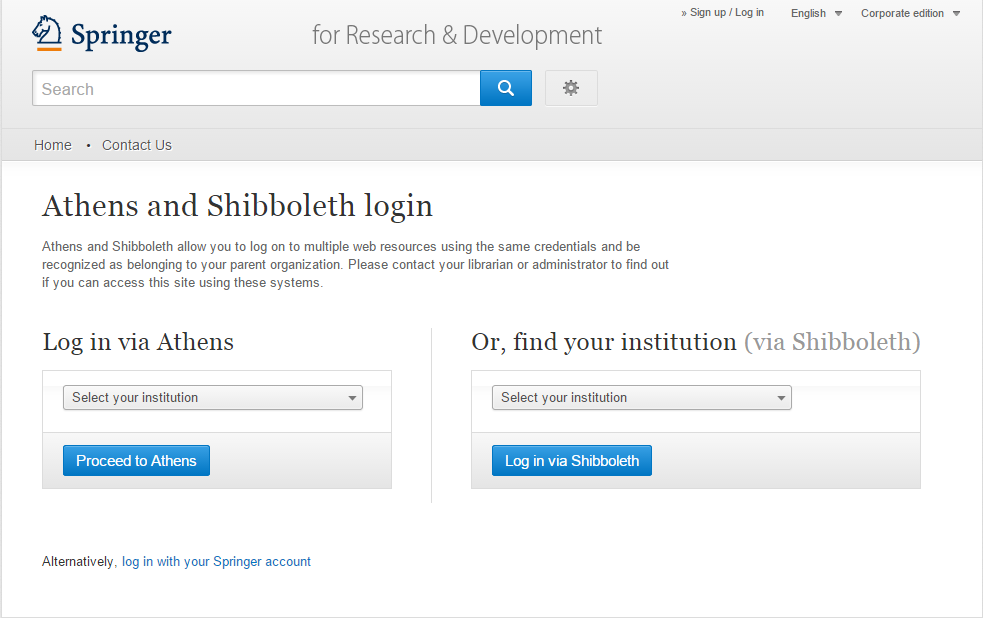
\includegraphics[width=8cm]{kapitel/gruppe2/bilder/springerlink_startseite}
	\caption{Springer Link Startseite \protect\footnotemark}
	\label{fig_springerlink_startseite}
\end{figure}\footnotetext{\url {http://link.springer.com/athens-shibboleth-login}, Abfragedatum: 30.05.2015}

\subsubsection{WISO}
Durch das Kooperationsverhältnis mit der GBI-Genios Deutsche Wirtschaftsdatenbank GmbH können die Mitglieder der Hochschule das komplette Angebot an Fachinformationen zu Wirtschafts- und Sozialwissenschaften, technischen Studiengängen und zur Psychologie  nutzen. WISO bietet über 14 Mio. Literaturnachweise, 2100 elektronische Bücher, 130 Mio. Artikel, 700.000 Marktdaten.\footnote{\url{https://www.wiso-net.de/popup/ueber_wiso}, Abfragedatum: 30.05.2015} Die WISO-Plattform ist in Abbildung \ref{fig_wiso_plattform.png} zu sehen.

\begin{figure}[h!]
	\centering
	\includegraphics[width=8cm]{kapitel/gruppe2/bilder/wiso_plattform.png}
	\caption{Übersicht der WISO-Plattform \protect\footnotemark}
	\label{fig_wiso_plattform.png}
\end{figure}\footnotetext{\url {https://www.wiso-net.de/}, Abfragedatum: 30.05.2015}

\subsubsection{video2brain}
Seit 2015 ist für alle Mitarbeiter und Studierende der Zugang zum Videostreaming-Portal der video2brain GmbH möglich. Schwerpunkt sind IT- und Kreativ-Themen, Lehrvideos für Fotografen, Grafiker, Web- und Screendesigner. Das Verlagsangebot umfasst mehr als 1700 Video-Trainingskurse. \footnote{vgl. \url{http://cmp.24-ads.com/de_DE/campaigns/detail/94}, Abfragedatum: 30.05.2015} In der Abbildung \ref{fig_video2brain_suchergebnis} ist die Weboberfläche nach erfolgreicher Shibboleth-Authentifizierung dargestellt.

\begin{figure}[h!]
	\centering
	\includegraphics[width=8cm]{kapitel/gruppe2/bilder/video2brain_suche}
	\caption{Übersicht der video2brain Plattform \protect\footnotemark}
	\label{fig_video2brain_suchergebnis}
\end{figure}\footnotetext{\url {https://www.video2brain.com/de/}, Abfragedatum: 30.05.2015}

\subsection{Support der Dienste}
Für die zentral angebotenen Dienste eduroam, Shibboleth und GigaMove übernimmt die Hochschule den Endkundensupport. Die Mitarbeiter der Hochschule bilden somit die zentrale Support-Schnittstelle und delegieren Anfragen, die vor Ort nicht gelöst werden können, an die entsprechenden Anbieter und Dienstleister weiter.

Diese teilte uns Günter Müller in dem durchgeführten Interview mit.